% =====================================================================
%  c08：原印刷页 64–71（PDF p.65–72）
%  §2.2.16、§2.2.17、§2.2.18（三者均为 2.2.x 三级标题，故用 \subsubsection；
%  父 \section 与 \subsection 在 c03 片段中定义，本片段不补）
%  片段开头是原书图 7、图 8 的图注页（这两张图的正文讨论在 c07 片段末尾），
%  故本片段第一行即插图；公式编号 (2.266)–(2.298) 连续无缺。
% =====================================================================

\begin{figure}[htbp]
  \centering
  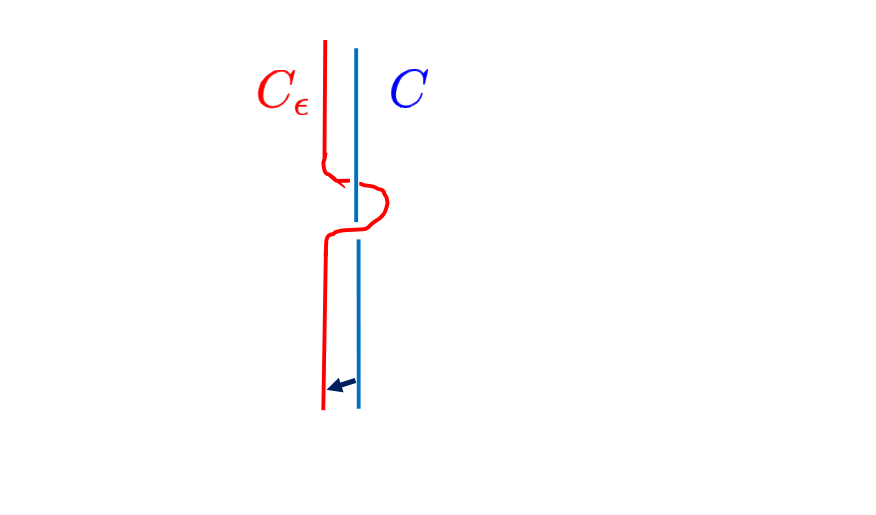
\includegraphics[width=0.45\textwidth]{figures/fig07.png}
  \caption{把 $C$ 沿法向作无穷小位移到 $C_\epsilon$，可能导致非平凡的自环绕，因为法向量可能绕着转。正因如此，$L(C,C)$ 是不良定义的。（原文 Fig.~7，第 64 页）}
  \label{fig:7}
\end{figure}

% 注意：figures/fig08.png 的裁切范围偏上，把图 7 的图形与其图注一并裁了进来（图 8 的图形在下方）。
% 此处按 brief 指定路径插入，未改动 figures/ 目录；若需出版质量，请重裁 fig08.png 后再编译。

\begin{figure}[htbp]
  \centering
  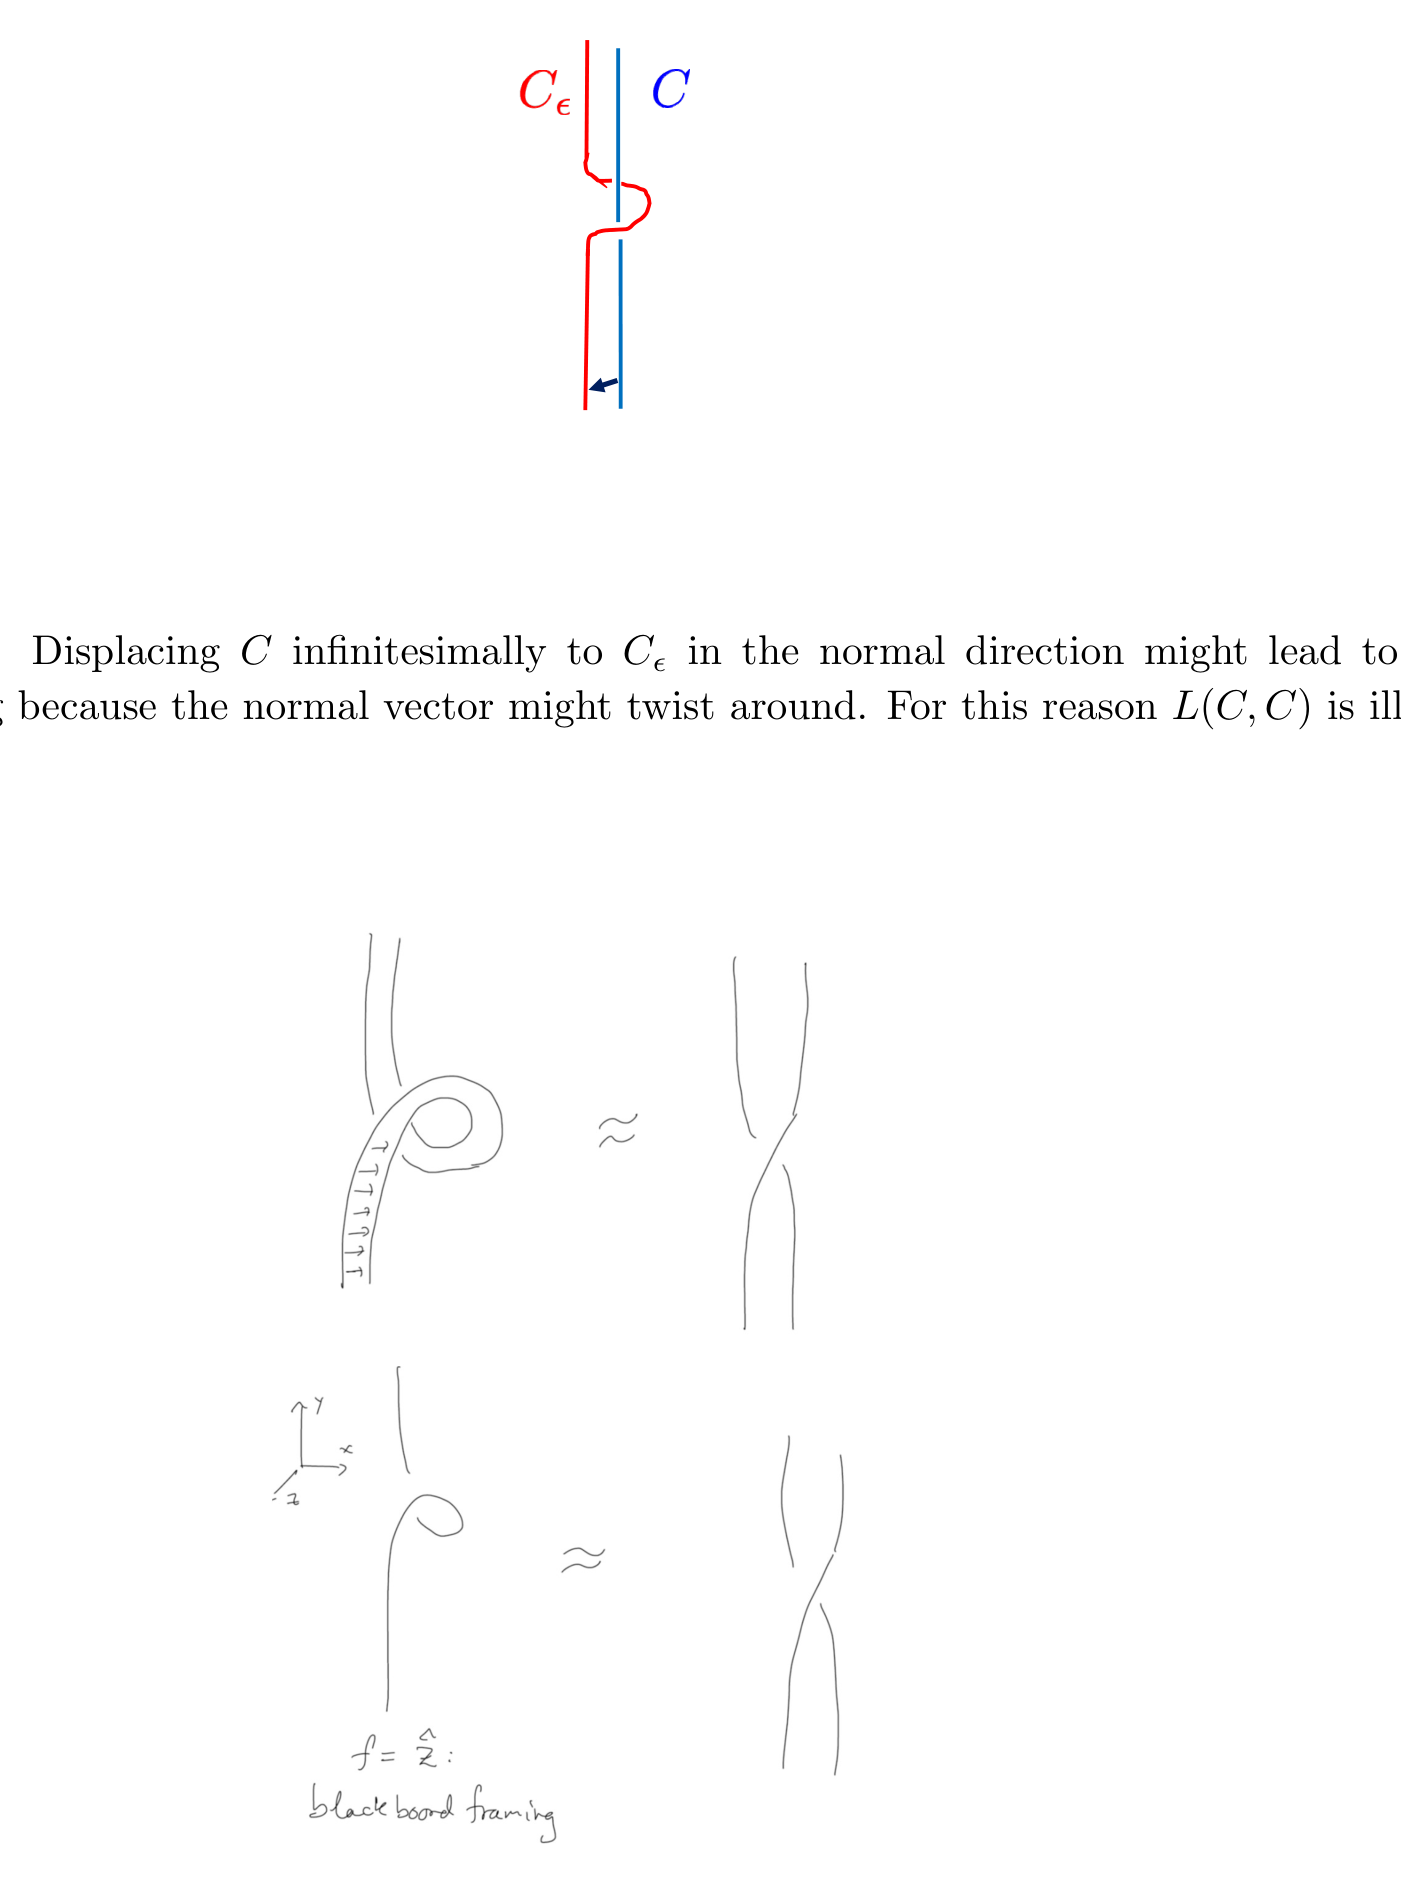
\includegraphics[width=0.55\textwidth]{figures/fig08.png}
  \caption{图示标架效应的不同但等价的画法。注意左下角：不加标架时，可以把绳子拉紧成一条直线。量子线缺陷依赖标架这一事实，会导致对第一 Reidemeister 移动的量子修正，如下文所述。（原文 Fig.~8，第 64 页）}
  \label{fig:8}
\end{figure}

\subsubsection{标架反常与缎带} % 原文: 2.2.16 The Framing Anomaly And Ribbons

以上所有讨论对 $\alpha\ne\beta$ 的那些项都运作良好。然而 $\alpha=\beta$ 时的环绕数还需要进一步讨论。正如自感（self-inductance）比互感（mutual inductance）要微妙得多，自环绕数也远比互环绕数微妙。自环绕数的公式显然在 Green 函数的重合点处有奇点。

这完全讲得通，正如图~\ref{fig:7} 所说明的。要定义 $L(C,C)$，必须把 $C$ 沿法向作无穷小位移，然后计算 $C$ 与其位移版本的互环绕数。但这显然是不良定义的，因为 $C$ 可能绕着自己转好几圈。在 Chern-Simons 理论中，这被称为\emph{标架反常}（framing anomaly）。

\textbf{定义}：\emph{Wilson 线算符的标架}（framing），是指 $\gamma\subset M_3$ 的法丛的一个处处非零截面，模去同伦（连续形变）。若 $s:\gamma\to N(\gamma)$ 是法丛的一个处处非零截面，我们就把标架记为 $f=[s]$。

更口语地说：我们可以说，在量子理论中 Wilson 线算符是与\emph{缎带}（ribbon）相联系的。当我们试图写出链环不变量时，这一点会有重要含义。预告见图~\ref{fig:8}。

\textbf{评注}

\begin{enumerate}
  \item 给定一个非零截面 $s:\gamma\to N(\gamma)$，我们可以把它拧上 $n$ 圈，$n$ 为任意整数。这里我们用到定向：Wilson 线是对一条定向曲线 $\gamma$ 定义的，因此垂直于线的圆盘上有确定的定向。于是拧 $n$ 圈就是在圆盘内作 $2\pi n$ 的逆时针旋转。注意这些标架并不构成 Abel 群：你不能把 $f_1+f_2$ 相加。因为若试图把法丛的两个截面相加，无法保证其和仍然非零。尽管如此，把一个整数加到一个标架上是有意义的：$f\to f+n$、$n\in\mathbb{Z}$；而且任意两个标架都可以通过这样的整数平移互相联系。数学上我们说，标架构成一个 $\mathbb{Z}$-torsor（$\mathbb{Z}$-主齐性空间）。\footnote{一般地，对任意群 $G$，若 $G$ 在集合 $S$ 上的作用既自由又传递，则称 $S$ 是一个 $G$-torsor。可以把 $S$ 想成 $G$ 的一份拷贝，只是没有选定单位元。主 $G$-丛的纤维就是 $G$-torsor 的好例子。}
  % [Tutor Note: 术语取舍。$G$-torsor 的中译常见「$G$-主齐性空间」与「$G$-扭子」两种，此处取前者，因为脚注 24 把它说成「未选单位元的 $G$ 的拷贝」，与主丛纤维的语义最贴；「扭子」又易与 twistor（扭量）相混。另注意作者特意强调标架不构成 Abel 群（不能相加 $f_1+f_2$），只能作 $\mathbb{Z}$-平移，这正是 torsor 与群的区别所在，写公式时务必用 $f+n$ 而不是 $f_1+f_2$。]

  \item 我们所发现的是：在 $W(r,\gamma)$ 的量子定义中，为了定义线缺陷，我们需要额外附加一份数据，即曲线 $\gamma$ 的标架。因此我们把记号改为
  \begin{equation}
    W(n,\gamma)\to W(n,\gamma,f)
    \tag{2.266}
    \label{eq:2.266}
  \end{equation}
  注意给定 $\gamma$ 与 $f$，存在良定义的同痕类 $\gamma+f$，而我们可以用
  \begin{equation}
    L_f(\gamma):=L(\gamma,\gamma+f)
    \tag{2.267}
    \label{eq:2.267}
  \end{equation}
  来定义自环绕数。因此，(2.255) 的一个更准确的版本是
  \begin{equation}
    \Big\langle\prod_{\alpha}W(r_{\alpha},\gamma_{\alpha},f_{\alpha})\Big\rangle
    =\mathcal{N}\cdot\exp\left[\sum_{\alpha<\beta}\frac{2\pi\mathrm{i}}{2\kappa}r_{\alpha}r_{\beta}L(\gamma_{\alpha},\gamma_{\beta})
    +\sum_{\alpha}\frac{2\pi\mathrm{i}}{4\kappa}r_{\alpha}^{2}L_{f_{\alpha}}(\gamma_{\alpha})\right]
    \tag{2.268}
    \label{eq:2.268}
  \end{equation}
  % [Tutor Note: (2.268) 的两个求和不能合并：$\sum_{\alpha<\beta}$ 只计互环绕，自环绕 $L_{f_\alpha}(\gamma_\alpha)$ 单列，且系数是 $\frac{2\pi\mathrm{i}}{4\kappa}$（比互环绕项的 $\frac{2\pi\mathrm{i}}{2\kappa}$ 多一个 $1/2$）。若把 $\sum_{\alpha<\beta}$ 写成 $\sum_{\alpha,\beta}$ 或 $\sum_{\alpha\le\beta}$，就会重复计数互环绕，并把自环绕项误算成互环绕项。自查办法：令所有 $\gamma_\alpha$ 互不链接、只各自带标架、且 $r_\alpha=n$，则 (2.268) 必须退化为纯相位 $\exp\big[\sum_\alpha\frac{2\pi\mathrm{i}}{4\kappa}n^{2}L_{f_\alpha}\big]$，与 (2.270) 在 $N=1$ 时一致。]

  \item 注意
  {\small\itshape ［原文标记：\ensuremath{\clubsuit} 会不会是 $-n$？需要核对。\ensuremath{\clubsuit}］}
  % [原文待办标记，原文 p.65 页边，作者对标架平移方向的正负号存疑]
  \begin{equation}
    L_{f+n}(\gamma)=L_f(\gamma)+n
    \tag{2.269}
    \label{eq:2.269}
  \end{equation}
  % [Tutor Note: 符号约定易错。(2.269) 里 $+n$ 对应「在法向圆盘内逆时针旋转 $2\pi n$」，作者自己在页边写「Could it be $-n$?」，说明他也没定下来。可靠的定号办法是从 (2.270) 反推：把 (2.269) 代入 (2.268) 的自环绕项，$f\to f+N$ 给出的比值必须是 $e^{2\pi\mathrm{i}Nn^{2}/(4\kappa)}$；若 (2.269) 取 $-n$，则该相位变号，「自旋为 $n^{2}/4\kappa$」这一物理解释随之翻转，与 (2.270) 不符。]

  因此
  \begin{equation}
    W(n,\gamma,f+N)=\left(e^{2\pi\mathrm{i}\frac{n^{2}}{4\kappa}}\right)^{N}W(n,\gamma,f)
    \tag{2.270}
    \label{eq:2.270}
  \end{equation}
  我们说 $e^{2\pi\mathrm{i}\frac{n^{2}}{4\kappa}}$ 是线缺陷的\emph{自旋}（spin）。（有些作者会说 $\frac{n^{2}}{4\kappa}\bmod\mathbb{Z}$ 是线缺陷的自旋。例如文献 [28] 就是在这个意义上使用的。当我们讨论与 RCFT 的关系时，这将与相应共形场的自旋、以及手征代数表示的量子维度联系起来。）

  \item 若 $\gamma\subset\Sigma_2$ 落在一个形如 $\Sigma_2\times\mathbb{R}$ 的 3-流形中，则我们可以把线缺陷 $W(n,\gamma,f)$ 视为 Hilbert 空间上的算符。若选取指向未来时间的自然标架，则该算符可以等同于我们在 Heisenberg 的故事里讨论过的算符 $\widehat{W}(n\gamma)$。

  \item \underline{线缺陷标号的等同}：注意 $n\to n+2\kappa$ 使关联函数不变。这与量子等同
  \begin{equation}
    W(n+2\kappa,\gamma,f)\cong W(n,\gamma,f)
    \tag{2.271}
    \label{eq:2.271}
  \end{equation}
  一致，后者是我们在考虑 Hilbert 空间 $\mathcal{H}(\Sigma_2)$ 上的算符时得到的。虽然相似，(2.271) 在概念上是不同的，因为它涉及的是插入路径积分中的线缺陷，而不是曲面物理 Hilbert 空间上的算符。

  从公式 (2.259) 我们看到，也可以通过给规范场施加边界条件来给出 Wilson 线可观测量的定义，而不是对光滑规范场作积分并添加源项（这是我们迄今一直做的）。从这个观点看，支撑在 $\gamma$ 上的线缺陷是这样定义的：挖掉 $\gamma$ 周围半径为 $\epsilon$ 的小管状邻域；而要定义荷为 $n$ 的缺陷，我们要求规范场满足这样的边界条件——若 $C(\epsilon)$ 是这个管状邻域边界上的小环绕曲线，则插入 $W(n,\gamma,f)$ 的路径积分具有边界条件
  \begin{equation}
    \lim_{\epsilon\to0}e^{\mathrm{i}\oint_{C(\epsilon)}A}=e^{-2\pi\mathrm{i}n/(2\kappa)}
    \tag{2.272}
    \label{eq:2.272}
  \end{equation}
  注意从这个观点看，我们自动得到等同 $n\sim n+2\kappa$。\footnote{这个论证有一个不严谨的版本如下：我们作一个奇异的规范变换，其变换函数在 Wilson 线附近形如 $g\sim e^{\mathrm{i}\phi}$，其中 $\phi$ 是方位角。Chern-Simons 作用量的改变量写作
  \begin{equation}
    \frac{\kappa}{2\pi}\int d(Ad\phi)+2\cdot\frac{\kappa}{2\pi}\int A\,d^{2}\phi
    \tag{2.273}
    \label{eq:2.273}
  \end{equation}
  这里我们说 $d(d\phi)=2\pi\delta^{(2)}(x)$，其中 $\delta^{(2)}(x)$ 是支撑在 Wilson 线上的 Dirac 测度。这个略显可疑的方程中的常数，是通过在一个圆盘上积分并施加 Stokes 定理得到的。在目前这个做法里没有边界，所以我们可以丢掉第一项。净效应是把 $n$ 平移为 $n+2\kappa$。}
  % [Tutor Note: (2.272) 的相位是 $e^{-2\pi\mathrm{i}n/(2\kappa)}$，而和乐 $e^{\mathrm{i}\oint A}$ 的周期是 $2\pi$，所以 $n$ 的模长是 $2\kappa$（与 (2.271) 的 $n\to n+2\kappa$、以及本节处处出现的荷格 $\mathbb{Z}/2\kappa\mathbb{Z}$ 一致），不是 $\kappa$。若把指数误写成 $e^{-2\pi\mathrm{i}n/\kappa}$，就会得到荷格 $\mathbb{Z}/\kappa\mathbb{Z}$，与 (2.271) 直接冲突。另外脚注 25 中 $2\cdot\frac{\kappa}{2\pi}\int A\,d^{2}\phi$ 的因子 2 来自 $d(A\,d\phi)=dA\,d\phi-A\,d^{2}\phi$ 的展开（$\phi$ 是角函数，$d^{2}\phi$ 是奇异的），核对时不要把它当成手误。]

  \item \underline{线缺陷的「算符乘积」}。一般地，当我们有「平行」缺陷时，我们想定义缺陷的「算符乘积」概念。在目前情形下，我们可以用 (2.268) 来定义 Wilson 线缺陷的算符乘积。为了定义我们所谓的「平行曲线」，我们假定 $\gamma_2$ 可由 $\gamma_1$ 经一次无穷小标架位移得到，从而 $\gamma_2$ 同痕于 $\gamma_1+f_{12}$。我们同样可以说 $\gamma_2=\gamma_1+f_{21}$。注意
  \begin{equation}
    L_{f_{12}}(\gamma_1)=L_{f_{21}}(\gamma_2)=L(\gamma_1,\gamma_2)
    \tag{2.274}
    \label{eq:2.274}
  \end{equation}
  现在考虑线缺陷的乘积：
  \begin{equation}
    W(n_1,\gamma_1,f_1)W(n_2,\gamma_2,f_2)
    \tag{2.275}
    \label{eq:2.275}
  \end{equation}
  假定所有其它线缺陷与 $\gamma_1$、$\gamma_2$ 的链接方式都相同，即
  \begin{equation}
    L(\gamma_1,\gamma_{\beta})=L(\gamma_2,\gamma_{\beta})\qquad\beta>2
    \tag{2.276}
    \label{eq:2.276}
  \end{equation}
  若 $\gamma_2$ 是由 $\gamma_1$ 经无穷小位移得到的，这一点自动成立。在条件 (2.276) 之下，我们可以把线缺陷的乘积 (2.275) 替换为单个线缺陷。为此我们写
  \begin{equation}
    \begin{aligned}
      f_1 &= f_{12}+N_{12}\\
      f_2 &= f_{21}+N_{21}
    \end{aligned}
    \tag{2.277}
    \label{eq:2.277}
  \end{equation}
  其中 $N_{12},N_{21}\in\mathbb{Z}$。于是有
  \begin{align}
    W(n_1,\gamma_1,f_1)W(n_2,\gamma_2,f_2)
      &\cong e^{2\pi\mathrm{i}\left(\frac{n_1^{2}}{4\kappa}N_{12}+\frac{n_2^{2}}{4\kappa}N_{21}\right)}W(n_1+n_2,\gamma_1,f_{12}) \notag\\
      &\cong e^{2\pi\mathrm{i}\left(\frac{n_1^{2}}{4\kappa}N_{12}+\frac{n_2^{2}}{4\kappa}N_{21}\right)}W(n_1+n_2,\gamma_2,f_{21})
    \tag{2.278}
    \label{eq:2.278}
  \end{align}

  \item \underline{单极子算符}。三维规范理论中一类重要的局域算符是单极子算符（monopole operator）。对具有规范群 $G$ 的一般规范理论，它们通过选取一个嵌入 $\mu:U(1)\to G$ 而得到。这允许把一个磁荷为 $\mu$ 的 Dirac 单极子嵌入 $G$ 规范理论，其中 $F^{\mathrm{Dirac}}=2\pi\frac{\sin\theta d\theta d\phi}{4\pi}$。然后我们可以在点 $p$ 处定义一个奇异的 $G$ 联络：用半径为 $\varepsilon$ 的小球包围 $p$，并要求当 $\varepsilon\to0$ 时
  \begin{equation}
    F\to\mu(F^{\mathrm{Dirac}})
    \tag{2.279}
    \label{eq:2.279}
  \end{equation}
  这个奇异的边界条件定义了一个荷为 $\mu$ 的点缺陷，即「单极子算符」$M_{\mu}(p)$。

  然而，若回想 Chern-Simons 作用量的规范变分 (2.45)，我们就会看到 $M_{\mu}(p)$ 不是规范不变的，而是按
  \begin{equation}
    M_{\mu}(p)\to e^{\mathrm{i}\kappa\mu(\epsilon(p))}M_{\mu}(p)
    \tag{2.280}
    \label{eq:2.280}
  \end{equation}
  变换。因此这个算符不是规范不变的。在一个非拓扑理论中，这个问题可以通过附加一条 Wilson 线、或乘上某个带相反荷的其它带电算符来补救；但在拓扑的 Chern-Simons 理论中，无法引入这些算符。

  {\small\itshape ［原文标记：\ensuremath{\clubsuit} 这里需要解释的东西还很多……\ensuremath{\clubsuit}］}
  % [原文待办标记，原文 p.67 页边]

  \item \underline{一形式对称性}。文献 [23] 中提出，量子场论里关于整体对称性的许多熟知事实，都能很好地推广为与更高维缺陷相联系的数学结构的变换。特别地，「一形式对称性」是与余维二维缺陷相联系的。当这些缺陷沿一条无穷小环绕与一维缺陷相链接时，结果是一个新的余维二维缺陷。这就是 [23] 的「一形式对称性」。在目前情形下，实现一形式对称性的对象本身就是那些一维缺陷，因而是 Wilson 线。它们构成一个同构于 $\mathbb{Z}/2\kappa\mathbb{Z}$ 的 Abel 群，这正是上述「算符乘积」下的群。由于上述简单的环绕规则，$W(n,\gamma)$ 在一形式对称群下的「荷为 $n$」。也就是说，它位于定义表示的第 $n$ 次幂之中。
  % 注：「第 $n$ 次幂」指 $W(n,\gamma)$ 同构于 $W(1,\gamma)$ 的 $n$ 重算符乘积；由 (2.271) 可知 $n$ 应读作 $\mathbb{Z}/2\kappa\mathbb{Z}$ 中的元素。

  \item {\small\itshape ［原文标记：COMMENT ON WHAT HAPPENS FOR WILSON LINES IN A GENERAL 3-MANIFOLD（评述一般 3-流形中 Wilson 线会发生什么）］}
  % [原文待办标记，原文 p.68：全大写，是作者留给自己的写作待办，正文内容尚未写出]
\end{enumerate}

\subsubsection{一个拓扑反常：归一化因子 $\mathcal{N}$} % 原文: 2.2.17 A Topological Anomaly: The Normalization Factor: N

如我们所说，归一化因子在形式上与度规无关，因为迄今为止我们并不需要使用度规。然而，要定义路径积分，我们必须对规范对称性作规范固定（gauge-fix），而任何规范固定的选择都会破坏路径积分形式上的拓扑对称性。所幸，拓扑不变性被破坏的方式是可计算的，而且这种破坏有很好的物理意义。

最标准的规范固定方式，是在 $M_3$ 上引入一个 Riemann 度规，并（在 Abel 情形）选取规范切片：
\begin{equation}
  d*A=\operatorname{vol}(g)g^{\mu\nu}D_{\mu}A_{\nu}=0
  \tag{2.281}
  \label{eq:2.281}
\end{equation}
这会把所有规范自由度固定到调和形式 $A\to A+\omega$ 为止。因此会剩下一个有限维环面 $\mathcal{H}^{0}(M_3;U(1))$ 的未固定规范变换。

标准的规范固定方式是在 BRST 步骤中引入 Faddeev-Popov 鬼场：我们引入反对易的零形式（取规范群的伴随表示）$c,b$，其鬼数分别为 $+1$、$-1$，并引入微分
\begin{equation}
  \begin{aligned}
    Q(A) &= Dc\\
    Q(c) &= 0\\
    Q(b) &= H\\
    Q(H) &= 0
  \end{aligned}
  \tag{2.282}
  \label{eq:2.282}
\end{equation}
并且我们往作用量里添加
\begin{equation}
  Q\Big(\mathrm{i}\int b\,d*A\Big)=\mathrm{i}\int b\,d*dc+\mathrm{i}\int H\,d*A
  \tag{2.283}
  \label{eq:2.283}
\end{equation}
我们应把 $H$ 看作 Lagrange 乘子。\footnote{通常在 BRST 步骤中会给 $H$ 加一个高斯项。但在目前情形下，那会破坏作用量的一阶（first-derivative）性质，并使这个漂亮的故事复杂化。} 对 $b,c$ 的积分给出
\begin{equation}
  \det' *d*d
  \tag{2.284}
  \label{eq:2.284}
\end{equation}
% [Tutor Note: 逻辑跳步。(2.283) 中没有通常的高斯项 $H^{2}$（脚注 26 说明：那会破坏作用量的一阶性质），所以 $H$ 是 Lagrange 乘子，对 $H$ 积分给出 $\delta(d*A)$ 而非高斯权重——这正是 (2.288) 里 Jacobian 的来源。另外 (2.284) 的 $\det'$ 来自对反对易场 $b,c$（鬼数 $+1,-1$，两者独立而非互为共轭）作 Grassmann 积分，结果是一个完整的行列式而不是平方根，带撇表示去掉零模；把它与 (2.289) 分母上的 $\det^{1/2}$ 对比时，务必分清哪个是 0-形式上的、哪个是 1-形式上的。作者在页边写「Should discuss zeromode」，正是指这个撇号尚未交代清楚。]

其中 $*d*d$ 是 0-形式上的标准度规 Laplacian。
{\small\itshape ［原文标记：\ensuremath{\clubsuit} 应讨论零模 \ensuremath{\clubsuit}］}
% [原文待办标记，原文 p.69 页边]

与此同时，我们可以把 Lagrange 乘子场重新标度为 $H=\text{const.}*\phi$，其中 $\phi\in\Omega^{3}(M_3)$，从而得到作用量
\begin{equation}
  \exp\Big[\frac{\mathrm{i}k}{2\pi}\int_{M_3}\big(AdA+\phi*d*A\big)
  =\exp\Big[\frac{\mathrm{i}k}{2\pi}\int_{M_3}\Phi*D\Phi\Big]
  \tag{2.285}
  \label{eq:2.285}
\end{equation}
% [Tutor Note: (2.285) 的括号在原文里就不配对（左端作 $\exp\big[\cdots\big($、右端作 $\big(\cdots\big]$），此处照原文转写；由右端形式可知左端应为 $\exp\big[\frac{\mathrm{i}k}{2\pi}\int_{M_3}(AdA+\phi*d*A)\big]$，这是原文的排版笔误。又：本小节 (2.285)–(2.290) 用的是斜体 $k$，而 (2.268) 等处用的是 $\kappa$，二者是同一个量（CS 能级／耦合常数），作者在此换了字母；不要把它当成第二个独立的耦合常数，否则 (2.289) 的 $2\pi\mathrm{i}k*d$ 与 (2.283) 的 $\frac{\kappa}{2\pi}$ 就无法配平。还有一处笔误：$\Phi*D\Phi$ 中的 $D$ 应即下面 (2.286) 的 $D_{+}$。]

其中
\begin{equation}
  \Phi=\begin{pmatrix}A\\ \phi\end{pmatrix}
  \qquad\qquad
  D_{+}=\begin{pmatrix}*d & 0 & 0\\ 0 & 0 & d*\\ 0 & d* & 0\end{pmatrix}
  \tag{2.286}
  \label{eq:2.286}
\end{equation}
这里
\begin{equation}
  D_{+}:\Omega^{\mathrm{odd}}(M_3)\to\Omega^{\mathrm{even}}(M_3)
  \tag{2.287}
  \label{eq:2.287}
\end{equation}
是 $D_{+}=*d+d*$。这可以解释为一个扭化 Dirac 算符（twisted Dirac operator）。当我们用非 Abel 理论重新审视这个计算时，会回到这一点。

后文在 ［原文标记：****］ 节中，我们会把 $D_{+}$ 看作扭化 Dirac 算符，并利用关于奇数维流形上 Dirac 算符行列式的一些一般事实。% [原文待办标记，原文 p.69：作者用「****」作节号占位，始终未填]
眼下我们改用一些 Hodge 理论。相关事实的综述见 F 节。算符 $*d:\Omega^{1}\to\Omega^{1}$ 是自伴的，\footnote{$(*d)^{\dagger}=d^{\dagger}*^{\dagger}=\pm*d**=\pm*d$。{\small\itshape ［原文标记：SIGN????（符号存疑）］}}% [原文待办标记，原文 p.69 脚注 27，作者对自己的符号推导存疑]
并且可以在 $\operatorname{Im}d^{\dagger}\subset\Omega^{1}$ 上对角化，谱为 $\mu_{n}^{(1)}$。这是一个类 Dirac 算符，其谱上下无界。与此同时，$\operatorname{Im}d\subset\Omega^{1}$ 上 $dd^{\dagger}$ 的谱为 $(\lambda_{n}^{(0)})^{2}$。

对 $H$ 的积分给出一个 delta 函数，于是我们得到一个 Jacobian
\begin{equation}
  \int_{\Omega^{1}}[dA]\,\delta(d*A)[\ldots]
  =\int_{\operatorname{Im}d^{\dagger}}[dA]\,\frac{1}{\prod_{n}|\lambda_{n}^{(0)}|}[\ldots]
  \tag{2.288}
  \label{eq:2.288}
\end{equation}
然后作剩下的积分给出行列式：
\begin{equation}
  \frac{\det' *d*d}{\det^{1/2}\Big(\frac{1}{2e^{2}}d^{\dagger}d+2\pi\mathrm{i}k*d\Big)\Big|_{\operatorname{Im}d^{\dagger}}}\;
  \frac{1}{\prod_{n}|\lambda_{n}^{(0)}|}
  \tag{2.289}
  \label{eq:2.289}
\end{equation}
第一个因子可以给出一个相位。我们用 $\zeta$-函数作正规化，于是
\begin{equation}
  \zeta(s)=\sum_{n}\Big(\frac{1}{2e^{2}}\big(\mu_{n}^{(1)}\big)^{2}+2\pi\mathrm{i}k\mu_{n}^{(1)}\Big)^{-s}
  \tag{2.290}
  \label{eq:2.290}
\end{equation}
注意存在谱不对称性。在 $e^{2}\to\infty$ 的极限下我们得到
\begin{equation}
  \operatorname{Im}\big(-\zeta'(0)\big)=\frac{\pi}{2}\eta(*d+d*)
  \tag{2.291}
  \label{eq:2.291}
\end{equation}
这给出了 CS 理论标架反常的一个漂亮的推导。

$\eta$ 不变量\emph{确实}有度规依赖，但这种度规依赖是局域的。我们会在 3.2.1 节用非 Abel 情形重新讨论这一点时再谈它。其绝对值为
\begin{equation}
  \prod_{n}\frac{|\lambda_{n}^{(0)}|}{\sqrt{|\mu_{n}^{(1)}|}}=\exp\Big[-\frac{1}{4}\tau(M_3)\Big]
  \tag{2.292}
  \label{eq:2.292}
\end{equation}
其中 $\tau(M_3)$ 是 Ray-Singer 挠率（Ray-Singer torsion），或称解析挠率。它是一个拓扑不变量，如附录 F 所示。
% [Tutor Note: (2.288) 的等号用到了 Hodge 分解 $\Omega^{1}=\operatorname{Im}d\oplus\operatorname{Im}d^{\dagger}\oplus\mathcal{H}^{1}$，以及 $d*A$ 在 $\operatorname{Im}d$ 上的 Jacobian 恰为 $\prod_{n}|\lambda_{n}^{(0)}|$；作者未写出这一步。再注意 (2.291) 的 $\eta$ 项（相位）与 (2.292) 的 $\tau$ 项（模长）是同一个行列式的两部分：$\tau$ 的定义本身就含 $\zeta'(0)$（除 $\eta$ 项外的对称部分），所以把两者相乘时不可重复计入 $e^{-\tau/4}$，也不可把 (2.291) 的 $\pi/2$ 与 (2.292) 的 $1/4$ 混用。]

\begin{figure}[htbp]
  \centering
  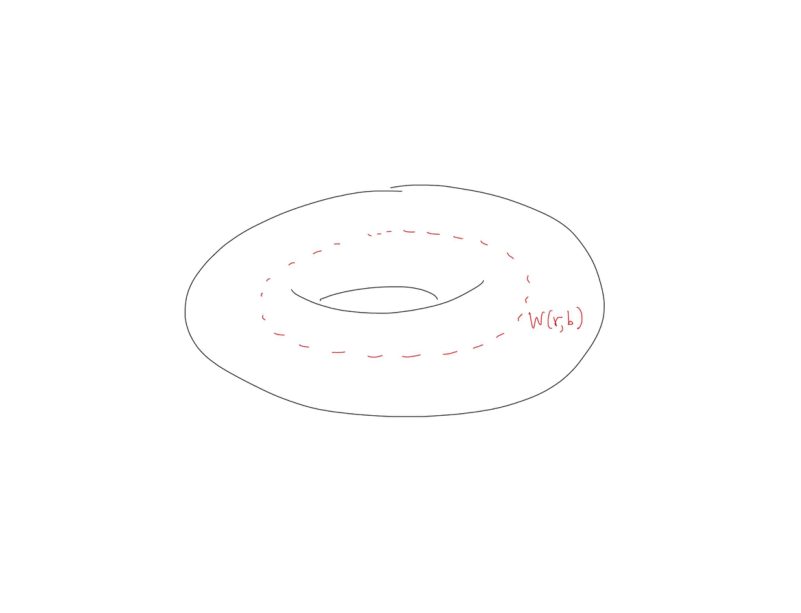
\includegraphics[width=0.55\textwidth]{figures/fig09.png}
  \caption{把手体上的路径积分（本图中是一个实心环面）定义了场之边界值的波泛函。在 Chern-Simons 理论的情形，它定义了围成该把手体的曲面的共形块空间中的一个特定状态。我们可以通过插入 Wilson 线缺陷这类非局域算符来改变该状态。（原文 Fig.~9，第 70 页）}
  \label{fig:9}
\end{figure}

\subsubsection{统一路径积分与 Hamilton 观点：由 Wilson 线生成的状态} % 原文: 2.2.18 Uniting The Path Integral And Hamiltonian Viewpoints: States Created By Wilson Lines

相当一般地，假设我们有一个 $d$ 维时空中的场论，场 $\phi$ 取值于某个靶空间 $\mathcal{T}$。若该理论由路径积分定义，那么当 $X$ 是一个 $d$ 维时空、其边界为 $\partial X=M$ 时，$X$ 上的路径积分就定义了与 $(d-1)$ 维流形 $M$ 相联系的 Hilbert 空间 $\mathcal{H}(M)$ 中的一个确定状态：
\begin{equation}
  \partial X=M\qquad\Rightarrow\qquad\psi_{X}\in\mathcal{H}(M).
  \tag{2.293}
  \label{eq:2.293}
\end{equation}
我们这里的记号是高度示意性的。例如，若我们在流形 $X$ 内部插入局域算符或其它缺陷，那就会改变我们所谓的 $X$ 是什么；而一般说来，这类插入肯定会使该状态改变。

方程 (2.293) 不难理解：为了定义路径积分，我们需要指定某些边界值 $\phi_\partial$，以便有合适的稳相近似和合适的经典变分问题。（$\phi_\partial$ 可能比场 $\phi$ 在 $\partial X$ 上的简单限制更为微妙。）我们可以把 $\mathcal{H}(M)$ 认定为边界条件空间上（适当可归一化的）波函数的空间，而具有特定边界条件 $\phi_\partial$ 的路径积分之值，被规定为状态 $\psi_X$ 在 $\phi_\partial$ 处的波函数值：
\begin{equation}
  \psi_X(\phi_\partial):=\mathit{PATH\ INTEGRAL\ WITH}\ \mathrm{b.c.}=\phi_\partial
  \qquad\Rightarrow\qquad
  \psi_X\in\mathcal{H}((M)
  \tag{2.294}
  \label{eq:2.294}
\end{equation}
% [Tutor Note: 原文 (2.294) 右端印作 $\mathcal{H}((M)$（多一个左括号、缺一个右括号），显系排版笔误，应为 $\mathcal{H}(M)$（与 (2.293) 一致）；此处照原文转写，以便与页面图像逐字对照。]

在基于「从几何范畴到张量范畴的函子」的场论公理化方法中，上述评述就变成了一条公理。（更确切地说，它是某些更基本公理的直接推论。）

把这一想法落实到目前 $U(1)$ Chern-Simons 理论的情形，做法如下。假设我们的 3-流形有一张边界曲面 $\Sigma_2$。先假定它是连通的。那么 3-流形 $M_3$ 就是所谓的把手体（handlebody）。注意存在群同态
\begin{equation}
  \iota:\pi_1(\Sigma_2,x_0)\hookrightarrow\pi_1(M_3,x_0)
  \tag{2.295}
  \label{eq:2.295}
\end{equation}
它诱导出同态
\begin{equation}
  \iota:H_1(\Sigma_2)\hookrightarrow H_1(M_3)
  \tag{2.296}
  \label{eq:2.296}
\end{equation}
这两个同态都会有很大的核：在图~3 中，如果我们按自然方式把曲面填满，那么所有 $a$-圈都映到零，而 $b$-圈保持非平凡。既然所有 $a$-圈都映到零，我们预期在算符方法里 $W(\gamma)\psi_{M_3}=\psi_{M_3}$ 对所有 $\gamma\in L_1$ 成立。这确实在 Stone-von Neumann 表示中挑出一条一维直线，从而挑出一个纯态。用该直线上某个非零向量 $\Psi_{M_3}$ 来表示这个态。

有意思的是，按上文建议的方式，通过插入一条荷为 $n_0\in\mathbb{Z}/2\kappa\mathbb{Z}$ 的 Wilson 线来改变 $X$，如图~\ref{fig:9} 所示。
{\small\itshape ［原文标记：\ensuremath{\clubsuit} 需要修图，使插入荷为 $n_0$ \ensuremath{\clubsuit}］}
% [原文待办标记，原文 p.71 页边]
一般地，我们可以考虑 $W(n_0\gamma)$，其中 $\gamma\in H_1(M_3;\mathbb{Z})$。这会产生一个新状态，它可以用非零向量 $\Psi_{M_3,n_0\gamma}$ 表示。设 $\hat\gamma\in H_1(\Sigma_2)$ 落在 $\iota$ 的原像中。显然
\begin{equation}
  \Psi_{M_3,n_0\gamma}=\widehat{W}(n_0\gamma)\Psi_{M_3}
  \tag{2.297}
  \label{eq:2.297}
\end{equation}
因为若把 Wilson 线施加到曲面上，我们可以让它「沉入」以获得图~\ref{fig:9} 中的图像。当然，这就是由下述条件确定的纯态（$\mathcal{H}(\Sigma_2)$ 中的一维直线）：它是 $W(\gamma')$ 的本征线，本征值为 $e^{2\pi\mathrm{i}\frac{\langle\gamma',n_0\gamma\rangle}{2\kappa}}$，对所有 $\gamma'\in L_b$ 成立。
\begin{equation}
  \widehat{W}(\gamma')\Psi_{M_3,n_0\gamma}
  =e^{2\pi\mathrm{i}\frac{\langle\gamma',n_0\gamma\rangle}{2\kappa}}\Psi_{M_3,n_0\gamma}
  \tag{2.298}
  \label{eq:2.298}
\end{equation}
事实上，(2.298) 也可以相当直接地推出：让 $\gamma'$ 同样「沉入把手体」，直到它与 $\gamma$ 相链接。

\begin{quote}
\small\itshape
［原文标记：***********************************************************

（1）讨论环面这一具体例子中的边界条件 $\phi_\partial$。

（2）现在推广到多个连通分支。它们的定向可以与 3-流形 $M_3$ 的定向一致或不一致，于是我们得到空间与对偶空间，即入射与出射空间。路径积分作为从入射到出射的线性变换。］
\end{quote}
% [原文待办标记，原文 p.71 页末：星号分隔的两条全大写写作提纲，作者尚未写成正文]

{\small\itshape ［原文标记：\ensuremath{\clubsuit} 需要修图：图中的表示应当画成缎带，且其标号是 $n_1$、$n_2$ 而不是 $\mu$、$\nu$ \ensuremath{\clubsuit}］}
% [原文待办标记，原文 p.71 页边]
